\begin{center}
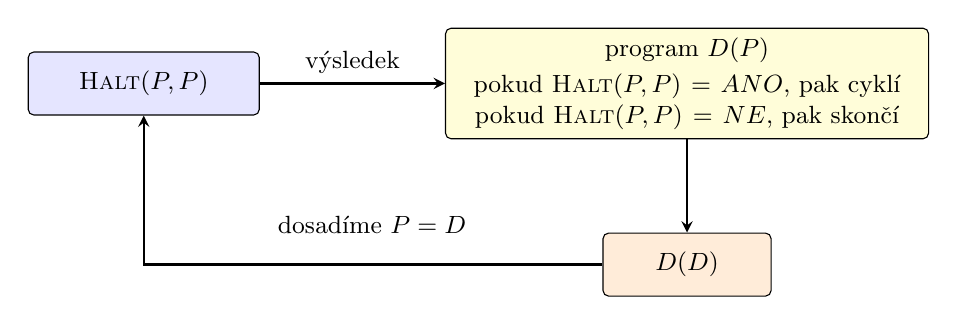
\begin{tikzpicture}[
    >=stealth,
    every node/.style={font=\small},
    box/.style={
        draw,
        rounded corners=2pt,
        align=center,
        minimum height=8mm
    }
]

% horní řada
\node[box, fill=blue!10, text width=2.7cm] (halt) at (0,0)
    {$\textsc{Halt}(P,P)$};

\node[box, fill=yellow!15, text width=5.9cm] (diag) at (6.9,0)
    {program $D(P)$\\[0.8mm]
     pokud $\textsc{Halt}(P,P)=\text{ANO}$, pak cyklí\\
     pokud $\textsc{Halt}(P,P)=\text{NE}$, pak skončí};

% dolní blok
\node[box, fill=orange!15, text width=1.9cm] (self) at (6.9,-2.3)
    {$D(D)$};

% vodorovná šipka z HALT do D(P)
\draw[->, thick] (halt.east) -- node[above] {výsledek} (diag.west);

% lomená šipka z D(P) do D(D)
\draw[->, thick]
    (diag.south) -- (self.north);

% lomená šipka z D(D) zpět do HALT
\draw[->, thick]
    (self.west) -- (2.4,-2.3) -| (halt.south);

% popisek k návratu
\node[align=center] at (2.9,-1.8) {dosadíme $P=D$};

% závěr
% \node[align=center] at (4.1,-3.35)
%     {Spor: $D(D)$ se zastaví právě tehdy, když se nezastaví.};

\end{tikzpicture}
\end{center}